\chapter{The exchanges in plain terms}\label{uch:exchanges}
Raven and MODFLOW exchange water in eight ways, and in a ninth when the soil zone is coupled
(Table~\ref{tab:uexchanges}). This chapter says what each exchange does, what controls it and what to write. Reference,
Chapter~\ref{R-ch:c4}, gives the equations, the safeguards and worked examples with numbers.

Figure~\ref{fig:uexch} shows where each exchange crosses between Raven and MODFLOW, and the table below lists them.
\begin{table}[!htbp]\centering
\caption{The exchanges between Raven and MODFLOW, and what switches them on.}\label{tab:uexchanges}\small
\begin{tabularx}{\linewidth}{P{0.2\linewidth}P{0.17\linewidth}P{0.2\linewidth}Y}\toprule\hdr
Exchange & Direction & Raven side & Switched on by\\\midrule
Recharge & Raven $\to$ aquifer & \cmd{GROUNDWATER} & always\\
Seepage & aquifer $\to$ Raven & lowest soil layer & always (existing model: \cmd{:SeepageToRaven ON})\\
Soil zone & both & soil-zone layers & \cmd{:SoilZone PHYSICAL}\\
Rivers & both & reach inflow & \cmd{:RiverGeometry} (existing model: \cmd{:StreamPackage})\\
Water-table ET & aquifer $\to$ air & unmet PET & \cmd{EXTINCTION\_DEPTH}~$>0$\\
Wetlands, lakes & both & HRU store & \cmd{:SurfaceWaterExchange}\\
Reservoirs & both & reservoir seepage & \cmd{:ReservoirExchange}\\
Wells & out (or in) & time series & \cmd{:Wells}\\
Boundaries & both & time series & \cmd{:GeneralHeadBoundary}, \cmd{:SpecifiedHeadBoundary}\\\bottomrule
\end{tabularx}\end{table}
\begin{figure}[!htbp]\centering% The exchanges between Raven and MODFLOW (both volumes of the manual)
\begin{tikzpicture}[x=1cm,y=1cm,lab/.style={font=\scriptsize,align=center},ar/.style={-{Stealth[length=2mm]},thick}]
\fill[orange!20] (0,0.8) rectangle (14,3.2); \fill[black!12] (0,0) rectangle (14,0.8);
\draw[thick,brown!60!black] (0,3.6) -- (2.8,3.6) -- (3.2,3.0) -- (4.2,3.0) -- (4.6,3.6) -- (7.6,3.6) -- (7.9,3.3) -- (9.3,3.3) -- (9.6,3.6) -- (14,3.6);
\fill[blue!25] (3.05,3.4) -- (4.35,3.4) -- (4.2,3.0) -- (3.2,3.0) -- cycle; \node[lab] at (3.7,4.05) {river};
\fill[cyan!20] (7.75,3.5) -- (9.45,3.5) -- (9.3,3.3) -- (7.9,3.3) -- cycle; \node[lab] at (8.6,4.05) {wetland / lake};
\draw[dashed,blue!70!black,thick] (0,3.3) .. controls (2,3.2) and (2.8,3.05) .. (3.7,3.1) .. controls (5,3.2) and (7,3.45) .. (8.6,3.5) .. controls (10,3.5) and (12,3.1) .. (14,2.9);
\node[lab,blue!70!black,anchor=west] at (1.25,2.8) {water table};
\draw[ar,teal!70!black] (1.0,4.6) -- node[lab,right]{recharge} (1.0,3.35);
\draw[ar,teal!70!black] (6.1,3.45) -- node[lab,right]{seepage} (6.1,4.5);
\draw[ar,blue!70!black,<->] (3.7,2.95) -- node[lab,right]{river exchange} (3.7,2.2);
\draw[ar,cyan!60!black,<->] (8.6,3.25) -- node[lab,right]{store exchange} (8.6,2.4);
\draw[ar,green!50!black] (10.9,3.25) -- node[lab,right]{water-table ET} (10.9,4.5);
\draw[thick] (13.2,4.7) -- (13.2,1.4); \draw[ar,red!70!black] (13.2,1.8) -- node[lab,left,pos=0.9]{well} (13.2,4.8);
\draw[ar,purple!70!black,<->] (0.1,1.7) -- node[lab,above]{GHB / CHD} (1.6,1.7);
\node[lab] at (7,1.6) {aquifer (MODFLOW)}; \node[lab] at (7,0.4) {bedrock};
\end{tikzpicture}

\caption{The exchanges between Raven (above the water table) and MODFLOW (below). Reservoir seepage works like the store
exchange, through Raven's reservoir seepage law.}\label{fig:uexch}
\end{figure}

\section{Recharge}\label{sec:urecharge}
Figure~\ref{fig:ulinking} shows how an HRU's water is shared among the cells under it.
\begin{figure}[!htbp]\centering% HRU over grid cells with its share in each cell (generated by make_tikz_linking.py; shares computed from the shapes)
\begin{tikzpicture}[x=1mm,y=1mm,font=\sffamily\footnotesize,every node/.append style={execute at begin node={\hyphenpenalty=10000\exhyphenpenalty=10000}}]
\node[anchor=south west,font=\sffamily\small] at (0,43) {(a) The HRU's share in each cell};
\fill[teal!18] (5.46,4.94) -- (19.50,3.64) -- (32.50,6.50) -- (46.80,4.29) -- (45.50,19.50) -- (47.58,34.06) -- (31.20,35.62) -- (19.50,32.76) -- (4.42,35.10) -- (6.76,19.50) -- cycle;
\draw[black!45,line width=0.4pt] (0,0) rectangle (13,13);
\draw[black!45,line width=0.4pt] (0,13) rectangle (13,26);
\draw[black!45,line width=0.4pt] (0,26) rectangle (13,39);
\draw[black!45,line width=0.4pt] (13,0) rectangle (26,13);
\draw[black!45,line width=0.4pt] (13,13) rectangle (26,26);
\draw[black!45,line width=0.4pt] (13,26) rectangle (26,39);
\draw[black!45,line width=0.4pt] (26,0) rectangle (39,13);
\draw[black!45,line width=0.4pt] (26,13) rectangle (39,26);
\draw[black!45,line width=0.4pt] (26,26) rectangle (39,39);
\draw[black!45,line width=0.4pt] (39,0) rectangle (52,13);
\draw[black!45,line width=0.4pt] (39,13) rectangle (52,26);
\draw[black!45,line width=0.4pt] (39,26) rectangle (52,39);
\draw[teal!70!black,line width=1.1pt] (5.46,4.94) -- (19.50,3.64) -- (32.50,6.50) -- (46.80,4.29) -- (45.50,19.50) -- (47.58,34.06) -- (31.20,35.62) -- (19.50,32.76) -- (4.42,35.10) -- (6.76,19.50) -- cycle;
\node[font=\sffamily\bfseries\scriptsize,text=teal!45!black,inner sep=0.5pt] at (9.37,8.21) {5\%};
\node[font=\sffamily\bfseries\scriptsize,text=teal!45!black,inner sep=0.5pt] at (9.67,22.57) {7\%};
\node[font=\sffamily\bfseries\scriptsize,text=teal!45!black,inner sep=0.5pt] at (9.10,30.37) {6\%};
\node[font=\sffamily\bfseries\scriptsize,text=teal!45!black,inner sep=0.5pt] at (19.17,8.35) {10\%};
\node[font=\sffamily\bfseries\scriptsize,text=teal!45!black,inner sep=0.5pt] at (19.50,19.50) {14\%};
\node[font=\sffamily\bfseries\scriptsize,text=teal!45!black,inner sep=0.5pt] at (22.24,29.67) {8\%};
\node[font=\sffamily\bfseries\scriptsize,text=teal!45!black,inner sep=0.5pt] at (29.53,9.47) {8\%};
\node[font=\sffamily\bfseries\scriptsize,text=teal!45!black,inner sep=0.5pt] at (32.50,19.50) {14\%};
\node[font=\sffamily\bfseries\scriptsize,text=teal!45!black,inner sep=0.5pt] at (31.56,30.78) {10\%};
\node[font=\sffamily\bfseries\scriptsize,text=teal!45!black,inner sep=0.5pt] at (42.70,8.71) {5\%};
\node[font=\sffamily\bfseries\scriptsize,text=teal!45!black,inner sep=0.5pt] at (42.43,22.47) {7\%};
\node[font=\sffamily\bfseries\scriptsize,text=teal!45!black,inner sep=0.5pt] at (43.05,30.47) {6\%};
\node[anchor=north,align=center,text width=50mm] at (26,-2) {One HRU (green) over 12 grid cells.\\The shares add up to 100\%.};
\node[anchor=south west,font=\sffamily\small] at (64,43) {(b) 10\,mm of recharge on a 5\,km$^2$ HRU};
\node[anchor=south west,align=left,inner sep=0pt] at (64,36.2) {Raven sends};
\fill[brand] (64,30.5) rectangle (112,35.5);
\node[anchor=west] at (113.5,33) {50\,000\,m$^3$};
\node[anchor=south west,align=left,inner sep=0pt] at (64,22.2) {Arrives if the weights are used as they are\\(here they add up to only 92\%)};
\fill[red!65!black] (64,16.5) rectangle (108.16,21.5);
\draw[red!65!black,pattern=north east lines,pattern color=red!65!black] (108.16,16.5) rectangle (112,21.5);
\node[anchor=west,text=red!65!black] at (113.5,19) {46\,000\,m$^3$ \ (4\,000\,m$^3$ lost)};
\node[anchor=south west,align=left,inner sep=0pt] at (64,8.2) {Arrives with Raven's shares, which always\\add up to 100\%};
\fill[teal!70!black] (64,2.5) rectangle (112,7.5);
\node[anchor=west] at (113.5,5) {50\,000\,m$^3$};
\end{tikzpicture}

\caption{Sharing an HRU's water among cells. (a) Raven computes the HRU's share in each cell from the shapes, and the shares add up to 100\%. (b) If the shares added up to only 92\%, 8\% of the water would be lost; because Raven's shares always add up to 100\%, every cubic metre arrives.}\label{fig:ulinking}
\end{figure}
Recharge is whatever Raven's processes put into the \cmd{GROUNDWATER} store of a coupled HRU during a step. Its volume is
that depth of water times the HRU's area in the \cmd{.rvh} file. Raven spreads it over the cells under the HRU, in
proportion to how much of the HRU lies in each cell, and hands it to MODFLOW the same step. Recharge that falls on
fixed-head cells goes to the fixed heads and is reported apart (\emph{recharge onto CHD cells}).

Recharge is therefore controlled by Raven's own process choices: percolation, infiltration, frozen ground and so on. The
coupling adds no control of its own.

\paragraph{Optional delay.} The profile parameter \cmd{RECHARGE\_DELAY} $\tau$ (days) holds recharge in a linear store
before it reaches MODFLOW. Each day the store releases the share $1-e^{-1/\tau}$ of its water; with $\tau=60$~d that is
1.65\% a day, and 63\% of a pulse has arrived after 60 days. With \cmd{:SoilZone PHYSICAL}, use an unsaturated column
(\cmd{:SoilZoneVadose LAG}) instead.

\section{Seepage back to Raven}\label{sec:useepage}
Figure~\ref{fig:ucurves} shows how four of the exchanges respond: a delayed recharge, the seepage near the land surface, a river, and evaporation from the water table.
\begin{figure}[!htbp]\centering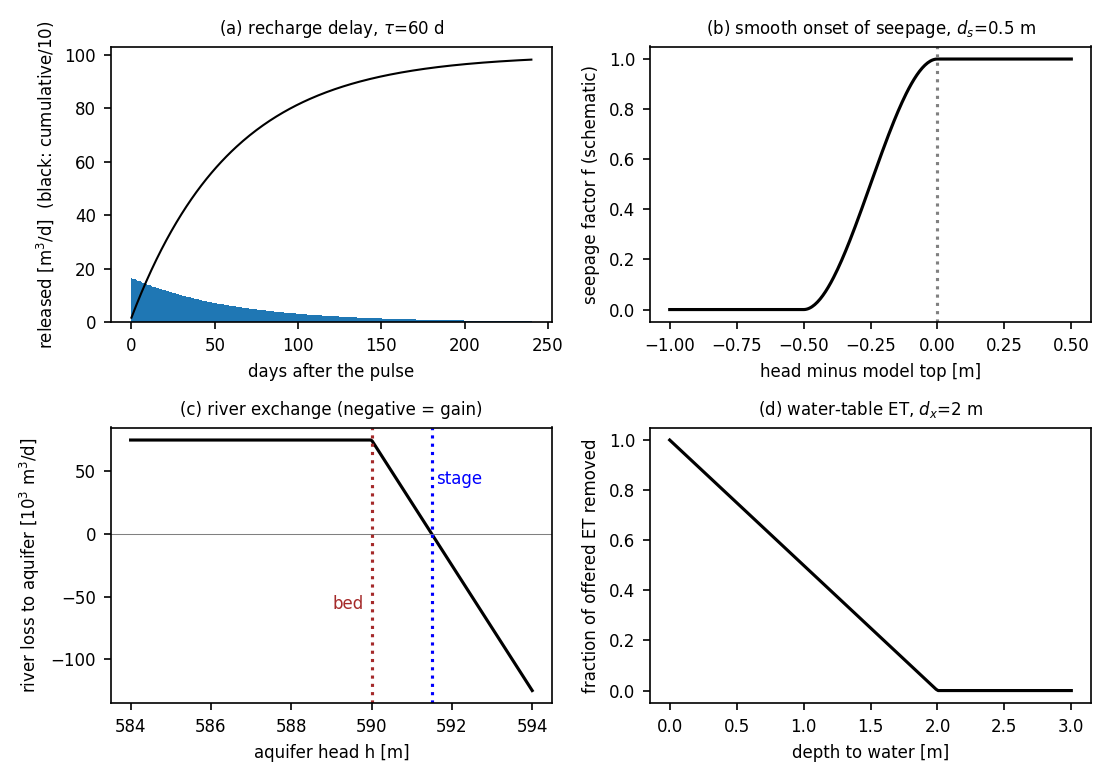
\includegraphics[width=\linewidth]{figures/fig_curves.png}
\caption{How four exchanges respond. (a) Recharge held in a delay reservoir reaches the aquifer gradually after a pulse of 1\,000~m$^3$. (b) Seepage starts as the water table nears the model top. (c) A river gains water when the aquifer head is above its stage and loses it when the head is below, at a limited rate once the water table drops below the river bed. (d) Evaporation from the water table is largest at the surface and stops at the extinction depth.}\label{fig:ucurves}
\end{figure}
Where the water table reaches the model top, groundwater flows out through a drain at the top of each cell. The drain
starts to flow \cmd{SEEPAGE\_SMOOTHING\_DEPTH} (default 0.5~m) below the top, and its strength is
\cmd{SEEPAGE\_LEAKANCE} (default 1/d) times the cell area. It is a strong outlet, so wherever the aquifer is full the water
table settles very close to the surface.

The seepage of a cell is returned to the HRUs above it, in proportion to their overlap, into the store named by
\cmd{:SeepageReturnTo}: by default the lowest soil layer, and \cmd{SURFACE\_WATER} for HRUs without soil. Raven's own
processes then carry it on, for example as baseflow to the river.

\section{Rivers}\label{sec:urivers}
Figure~\ref{fig:uriver} shows a river cell.
\begin{figure}[!htbp]\centering
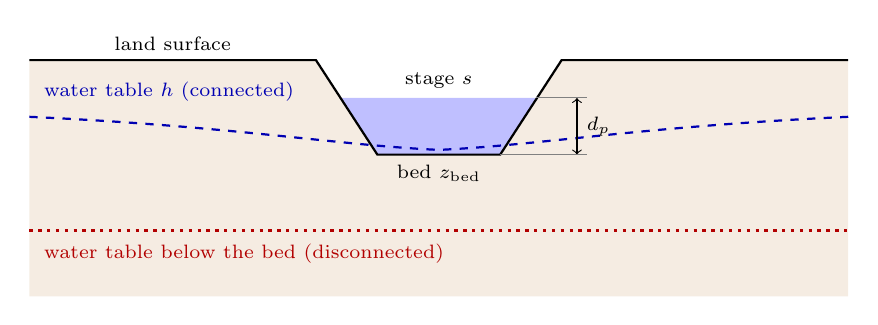
\begin{tikzpicture}[x=1.3cm,y=1.2cm,lab/.style={font=\scriptsize}]
\fill[brown!15] (-4,0) -- (4,0) -- (4,2.5) -- (1.2,2.5) -- (0.6,1.5) -- (-0.6,1.5) -- (-1.2,2.5) -- (-4,2.5) -- cycle;
\fill[blue!25] (-0.95,2.1) -- (0.95,2.1) -- (0.6,1.5) -- (-0.6,1.5) -- cycle;
\draw[thick] (-4,2.5) -- (-1.2,2.5) -- (-0.6,1.5) -- (0.6,1.5) -- (1.2,2.5) -- (4,2.5);
\draw[dashed,blue!70!black,thick] (-4,1.9) .. controls (-2,1.8) and (-1,1.6) .. (0,1.55) .. controls (1,1.6) and (2,1.8) .. (4,1.9);
\node[lab,blue!70!black,anchor=west] at (-3.95,2.17) {water table $h$ (connected)};
\draw[dotted,red!70!black,very thick] (-4,0.7) -- (4,0.7); \node[lab,red!70!black,anchor=west] at (-3.95,0.45) {water table below the bed (disconnected)};
\draw[<->] (1.35,1.5) -- (1.35,2.1); \node[lab,right] at (1.35,1.8) {$d_p$};
\draw[gray,thin] (0.6,1.5) -- (1.45,1.5); \draw[gray,thin] (0.95,2.1) -- (1.45,2.1);
\node[lab] at (0,2.28) {stage $s$}; \node[lab] at (0,1.3) {bed $z_{\mathrm{bed}}$};
\node[lab,anchor=south] at (-2.6,2.5) {land surface};
\end{tikzpicture}

\caption{A river cell. The river's stage is its bed plus the channel depth Raven computes. While the water table is above the bed, water flows toward the lower of the two levels; once the water table drops below the bed, the river loses water at a rate that no longer grows as the water table falls.}\label{fig:uriver}
\end{figure}
Rivers exchange water with the aquifer in both directions. A \emph{gaining} river receives groundwater; a \emph{losing}
river leaks into the aquifer. Raven places a river cell (MODFLOW's RIV package) in every cell crossed by a river line of
\cmd{:RiverGeometry}. The exchange of a river cell is
\[
q = C\,(s-h),
\]
where $q$ is the flow from the river into the aquifer [m$^3$/d], $s$ the river level, $h$ the head of the cell, and $C$
the riverbed conductance: the riverbed conductivity \cmd{RIVERBED\_K} times the river's width and length in the cell,
divided by the riverbed thickness \cmd{RIVERBED\_THICKNESS}. When the head falls below the riverbed, the loss stops
growing: $h$ is replaced by the bed elevation.

\begin{itemize}
\item \textbf{The riverbed} lies one bankfull depth of Raven's channel (at its reference flow) below the lowest DEM value
along the river in the cell, or \cmd{:RiverBedDepth} metres below it.
\item \textbf{The river level} each day is the bed plus Raven's channel depth at the start of the day, never above the
land surface.
\item \textbf{A gain} is added to the subbasin's inflow for the day, so it passes Raven's routing like other runoff.
\item \textbf{A loss} (the \emph{river-loss take}) is taken from the subbasin's own inflow, then from the flow entering the
reach from upstream, then from the reach's outflow. The outflow leaving the watershed is lower by exactly the water
MODFLOW receives.
\end{itemize}
\begin{example}[: a river cell]
Riverbed conductivity 0.5~m/d, riverbed 1~m thick, river 40~m wide, 2\,500~m of river in the cell:
$C=0.5\times40\times2\,500/1=50\,000$~m$^2$/d. Bed at 590~m, river 1.5~m deep, so the river level is 591.5~m.
With the water table at 590.8~m the river loses $50\,000\times0.7=35\,000$~m$^3$/d to the aquifer. With the water table
at 592.0~m it gains 25\,000~m$^3$/d. With the water table at 585~m, below the bed, it loses
$50\,000\times1.5=75\,000$~m$^3$/d, and no more however low the water table falls.
\end{example}

\paragraph{A river cannot lose more than it carries.} Raven limits the conductance of each river cell every day, so that
the largest possible loss is no more than the cell's share (by river length) of the flow in the reach at the start of
the day. Only a reach whose flow stops within the step can leave part of its loss unpaid; that part is carried to the next
step (\emph{river loss carried to next step}, normally 0; Raven warns). An existing model's stream package has no such
limit (Chapter~\ref{uch:existing}).

\begin{inpractice}
Calibrate \cmd{RIVERBED\_K} and \cmd{:RiverBedDepth} on the grid you will use: the river exchange depends on the size of the
river cells (Section~\ref{sec:liardgrids}).
\end{inpractice}

\section{Evaporation from a shallow water table}\label{sec:uet}
Plants and bare soil can draw water from a water table close to the surface. With the profile parameter
\cmd{EXTINCTION\_DEPTH} greater than 0, MODFLOW's EVT package is added. Raven first meets evaporation from its own stores.
Only the potential evaporation it could \emph{not} meet is offered to the water table. The rate falls linearly from that
unmet demand, with the water table at the top, to zero, with the water table at the extinction depth. Only HRUs whose own
profile has an extinction depth take part.
\begin{example}[: water-table evaporation]
Unmet potential evaporation 2~mm/d over a 4~km$^2$ cell fully covered by coupled HRUs, extinction depth 2~m, water table
0.5~m deep: $0.002\times4\times10^6\times(1-0.5/2)=6\,000$~m$^3$/d evaporate from the water table.
\end{example}

\section{Wetlands and lakes held in Raven stores}\label{sec:ustores}
Wetlands and small lakes are often a store in their HRUs: \cmd{DEPRESSION} for wetlands, \cmd{LAKE\_STORAGE} for lakes.
\begin{whattowrite}
\cmd{:SurfaceWaterExchange DEPRESSION WetlandHRUs LEAKANCE 0.01}\quad (\cmd{.rvg}; the store, an HRU group, a leakance in 1/d)
\end{whattowrite}
connects that store, in the HRUs of the group, to the aquifer below. The exchange works like a river whose bed is the model
top and whose level is the top plus the depth of water in the store. Water leaks down when the store holds water above
a lower water table; groundwater flows up into the store when the water table is higher. The leak is limited so that it
never drains more than the store holds.

\section{Reservoirs}\label{sec:ureservoirs}
Raven reservoirs can already lose water through their \cmd{:SeepageParameters}: a seepage constant and a fixed
groundwater level. \cmd{:ReservoirExchange} (\cmd{.rvg}) replaces that fixed level by the aquifer head below the lake, for
every reservoir that has \cmd{:SeepageParameters} and whose lake HRU (\cmd{:HRUID}) has an \cmd{AQUIFER\_PROFILE}. The
seepage computed in one step is injected into the aquifer under the lake the next step; the water in transit is reported
and saved for restarts.
\begin{watch}
The reservoir stage and the aquifer heads must use the same vertical datum. Give reservoirs absolute elevations (for
simple lakes, \cmd{:AbsoluteCrest\allowbreak Height}) and an initial stage or flow in the \cmd{.rvc} file
(\cmd{:InitialReservoirStage} or \cmd{:InitialReservoirFlow}): without either Raven starts the reservoir at stage 0 and
fills it in the first step, a jump in Raven's water balance (a warning says so). A stage below the whole aquifer under
the lake after the first step stops the run. The lake HRU (\cmd{:HRUID}) must lie in the reservoir's own subbasin;
otherwise Raven crashes in its first step (also without groundwater), and the coupled model stops with a message
instead.
\end{watch}

\section{Wells and boundaries}
Wells pump from the aquifer (or inject into it), and head boundaries exchange water with water bodies outside the model.
Pumped water leaves the system; Figure~\ref{fig:upumping} shows a pumping test. Section~\ref{sec:uwells} says what to write. A well placed in a fixed-head cell has no
effect, and Raven warns about it.

Pumped water comes at first mostly from aquifer storage. As the cone of depression reaches rivers and seepage areas, more
and more of it comes from reduced discharge to streams (``capture''). In the Liard pumping test 91\% of the pumping was
captured from reduced discharge to rivers in the first year and 98\% in the fifth (Reference, Section~\ref{R-ch:wells}).
\begin{figure}[!htbp]\centering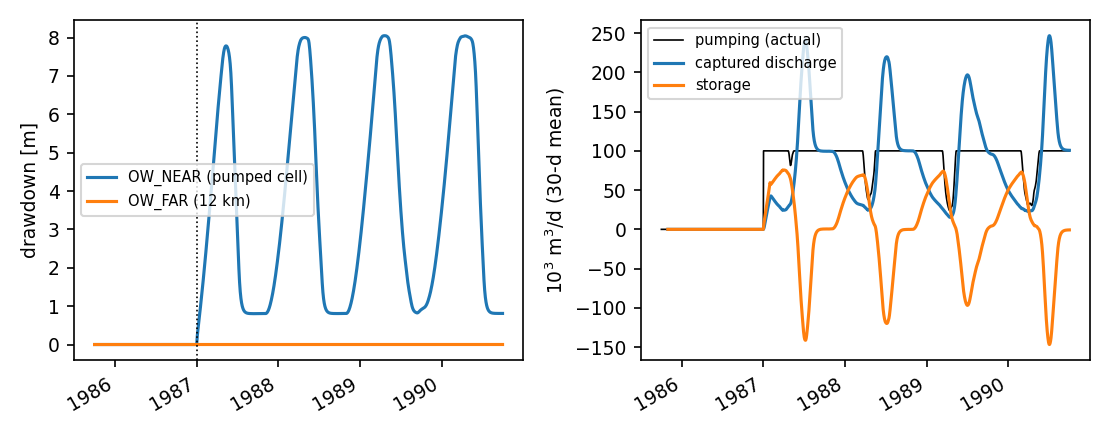
\includegraphics[width=\linewidth]{figures/fig_pumping.png}
\caption{Pumping test: drawdown at the monitoring wells (left) and where the pumped water comes from (right).}\label{fig:upumping}
\end{figure}

\section{The soil zone: CONCEPTUAL or PHYSICAL}\label{sec:usoilzone}
By default (\cmd{:SoilZone CONCEPTUAL}) Raven's soil and the aquifer meet only through recharge and the seepage drain:
Raven's soil never sees the water table.

With \cmd{:SoilZone PHYSICAL} the soil layers you name become the top of the aquifer, owned by Raven. MODFLOW starts below
them. The water table can rise into them: saturated soil drains to the aquifer, recharge stops where the ground is
saturated, and a full soil zone overflows to the surface. This is the arrangement of GSFLOW
\cite{markstrom2008gsflow}.

\begin{plain}
Think of the soil layers you name (for example \cmd{SOIL[0]} and \cmd{SOIL[1]}) as the top of the aquifer, owned by
Raven. MODFLOW starts below them. When the water table climbs to the bottom of the soil, it carries on rising inside the
soil layers; rain falling on that saturated ground cannot soak down any more and stays in the soil, and once the soil is
full the extra water runs off. When it is dry, saturated soil drains down into the aquifer again. On a slope this
happens first at the bottom of the hill, because Raven checks the ground height at many points in each cell.
\end{plain}

\begin{table}[!htbp]\centering
\caption{Which soil-zone option to use.}\label{tab:uszchoice}
\begin{tabularx}{\linewidth}{P{0.25\linewidth}Y}\toprule\hdr
Option & Use it when\\\midrule
\cmd{CONCEPTUAL} (default) & the water table stays below the soil, or for a first model\\
\cmd{PHYSICAL} & the water table reaches the soil: valley floors, wetlands, the foot of slopes, flat lowlands. It takes more computing time per day\\\bottomrule
\end{tabularx}
\end{table}

\subsection{A water table in the soil, on sloping and irregular land}\label{sec:applysz}
On irregular land the water table meets the soil in some parts of a cell and not in others (Figure~\ref{fig:uszsubgrid}).
\begin{figure}[!htbp]\centering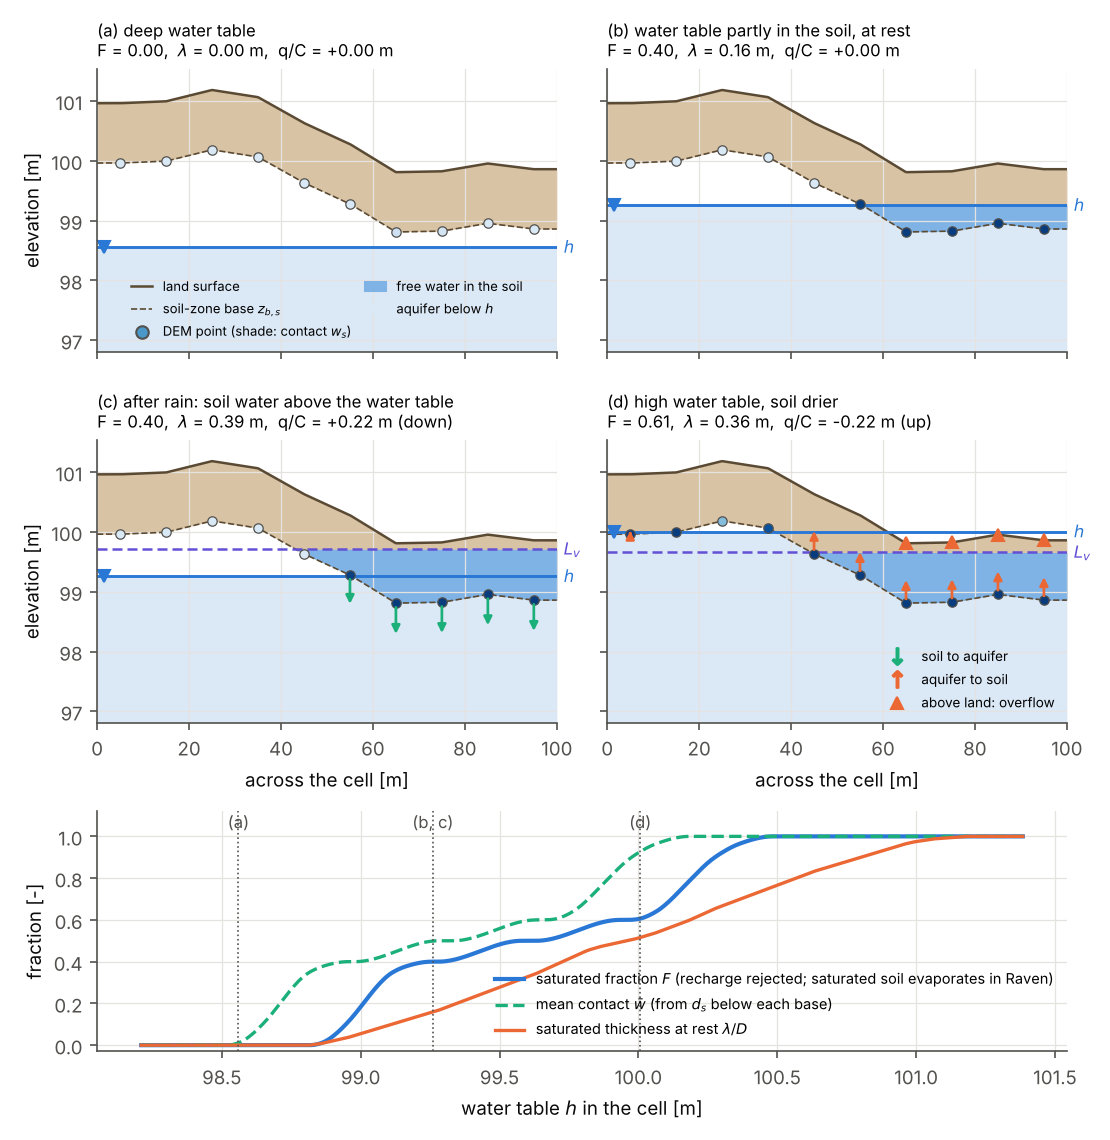
\includegraphics[width=\linewidth]{figures/fig_sz_subgrid.png}
\caption{One 100~m cell with irregular land. Raven samples the land inside each cell at many points (circles). (a) to (d): four positions of the water table and of the water in the soil; the arrows show how much of the exchange between soil and aquifer each point carries, and only the part of the cell where the water table reaches the soil (the saturated fraction) is wet. Bottom: that fraction against the water table.}\label{fig:uszsubgrid}
\end{figure}
Figure~\ref{fig:uszregimes} shows every position the water table can take, and what carries the water in each.
\begin{figure}[!htbp]\centering% Positions of the water table relative to the soil zone and what carries the water in each
\begin{tikzpicture}[font=\sffamily\scriptsize,x=1mm,y=1mm,
  soil/.style={fill=brown!18,draw=brown!60!black,line width=0.4pt},
  unsat/.style={fill=yellow!10,draw=none},
  sat/.style={fill=blue!12,draw=none},
  wt/.style={blue!70!black,line width=1.1pt},
  base/.style={brown!60!black,dashed,line width=0.6pt},
  up/.style={-{Stealth[length=1.8mm]},line width=0.8pt,teal!70!black},
  dn/.style={-{Stealth[length=1.8mm]},line width=0.8pt,orange!85!black},
  lab/.style={align=center,text width=23mm,inner sep=1pt}]
% one panel: x offset #1, water-table elevation #2 (land 60, soil base 48, soil layers 48-54-60)
\newcommand{\panel}[2]{%
  \fill[sat] (#1,0) rectangle (#1+26,#2);
  \fill[unsat] (#1,#2) rectangle (#1+26,48);
  \draw[soil] (#1,48) rectangle (#1+26,54);
  \draw[soil] (#1,54) rectangle (#1+26,60);
  \draw[base] (#1,48) -- (#1+26,48);
  \draw[line width=0.8pt] (#1,60) -- (#1+26,60);
  \draw[gray] (#1,0) rectangle (#1+26,60);}
% (a) deep water table
\panel{0}{14}
\draw[wt] (0,14) -- (26,14); \fill[blue!70!black] (21,14) -- ++(-1.4,2.2) -- ++(2.8,0) -- cycle;
\draw[dn] (4,47) -- (4,17); \node[lab,text width=13mm,align=left,anchor=west] at (5,36) {Richards column: delay, spreading};
\draw[up] (22,17) -- (22,49.5); \node[lab,text width=12mm,align=right,anchor=east] at (20.8,23) {rise from the column};
% (b) just below the soil base
\panel{30}{45}
\draw[wt] (30,45) -- (56,45); \fill[blue!70!black] (51,45) -- ++(-1.4,2.2) -- ++(2.8,0) -- cycle;
\draw[up] (37,45.5) -- (37,57); \draw[up] (42,45.5) -- (42,51);
\node[lab] at (43,32) {steady capillary rise from the water table into every layer below field capacity; contact through the fringe $d_s$};
% (c) in the soil zone
\panel{60}{52}
\fill[sat] (60,48) rectangle (86,52); \draw[wt] (60,52) -- (86,52); \fill[blue!70!black] (81,52) -- ++(-1.4,2.2) -- ++(2.8,0) -- cycle;
\draw[up] (66,52.5) -- (66,58.5);
\draw[{Stealth[length=1.8mm]}-{Stealth[length=1.8mm]},line width=0.8pt,violet] (73,44) -- (73,51);
\node[lab] at (73,28) {saturated soil exchanges with the aquifer (Robin interface); recharge rejected on saturated ground; rise into the layer above};
% (d) at the land surface
\panel{90}{60}
\fill[sat] (90,48) rectangle (116,60); \draw[wt] (90,60) -- (116,60);
\node[lab] at (103,32) {full soil zone overflows to SURFACE\_\-WATER: rain and exfiltration run off the same day};
% (e) specified head
\panel{120}{50}
\fill[sat] (120,48) rectangle (146,50); \draw[wt,dash pattern=on 3pt off 1.5pt] (120,50) -- (146,50);
\draw[{Stealth[length=1.8mm]}-{Stealth[length=1.8mm]},line width=0.8pt,violet] (133,43) -- (133,49.5);
\node[lab] at (133,32) {fixed head: exact exchange of each column with the head, no MODFLOW boundary};
% labels
\foreach \x/\t in {0/(a) deep,30/(b) below the base,60/(c) in the soil zone,90/(d) at the surface,120/(e) specified head}{
  \node[font=\sffamily\bfseries\scriptsize,anchor=south] at (\x+13,61) {\t};}
\node[anchor=east,font=\sffamily\tiny] at (-0.5,57) {SOIL[0]}; \node[anchor=east,font=\sffamily\tiny] at (-0.5,51) {SOIL[1]};
\node[anchor=east,font=\sffamily\tiny,brown!60!black] at (-0.5,47) {base}; \node[anchor=east,font=\sffamily\tiny] at (-0.5,8) {aquifer};
\end{tikzpicture}

\caption{Where the water table can be and what moves the water in each case. (a) Deep: recharge crosses an unsaturated
column solved with Richards' equation (\cmd{:SoilZoneVadose RICHARDS}), which delays and spreads it; the column also
feeds capillary rise into the soil zone. (b) Within the column's minimum length below the soil base: no column; the
exchange starts through the fringe $d_s$, and capillary rise from the water table reaches the layers above. (c) In the
soil zone: the saturated soil exchanges with the aquifer, recharge on saturated ground is rejected, capillary rise
continues into the layers above the water table. (d) At the surface: the full soil zone overflows. (e) Over a specified
head: each column exchanges with the fixed head exactly.}\label{fig:uszregimes}
\end{figure}
Where the water table comes close to the land --- valley bottoms, the foot of slopes, wetlands, flat lowlands --- add the
soil zone: the water table can then rise into Raven's soil layers, saturated ground rejects recharge, groundwater
discharges into the soil, and full soil overflows to surface water. Nothing else of the model changes.
\begin{enumerate}
\item \textbf{Choose the soil-zone layers} (\cmd{.rvg}): the physical soil layers above the aquifer, usually the top one
or two, \cmd{:SoilZone PHYSICAL SOIL[0] SOIL[1]}. MODFLOW's top then lies one soil-zone thickness below the land, cell by
cell, so the model's top follows the slope.
\item \textbf{Send recharge from the bottom soil-zone layer} (\cmd{.rvi}): for example
\cmd{:Percolation PERC\_GAWSER SOIL[1] GROUNDWATER}, conditional on the coupled HRUs. A drainage that moves only water above
field capacity lets a soil zone that is not connected to the water table pass the rain on.
\item \textbf{Soil parameters} (\cmd{.rvp}): \cmd{POROSITY}, \cmd{FIELD\_CAPACITY} ($<1$), and \cmd{HYDRAUL\_COND} [mm/d] for
the class of the bottom soil-zone layer; \cmd{CLAPP\_B} and \cmd{AIR\_ENTRY\_PRESSURE} for capillary rise. Give the top
aquifer layer a specific yield close to the soil's drainable porosity, $\eta(1-S_{\mathrm{fc}})$ (porosity $\eta$ times
one minus the field capacity $S_{\mathrm{fc}}$): otherwise the water table rises at different rates below and inside the
soil (Raven warns).
\item \textbf{Sloping and irregular land}: give a DEM finer than the cells. Each cell samples it at
\cmd{:SoilZoneSubgrid} $n$ points per side (5 by default, 25 points), so within a cell the low ground saturates first
and the high ground later (Reference, Figure~\ref{R-fig:szsubgrid}; Figure~\ref{fig:uszhillslope} shows a coupled hillslope). Between cells MODFLOW's heads carry the water down
the slope, and the saturated area spreads up from the foot of the slope and from hollows and retreats downslope as it
dries (Reference, Figure~\ref{R-fig:szhillslope}). Keep \cmd{SEEPAGE\_SMOOTHING\_DEPTH} (the contact depth $d_s$) at
0.1--0.5~m. Seepage faces and saturated strips narrower than a cell need smaller cells (or \cmd{:GridRefinement} along
valleys); within a cell the soil water stands at one level.
\begin{figure}[!htbp]\centering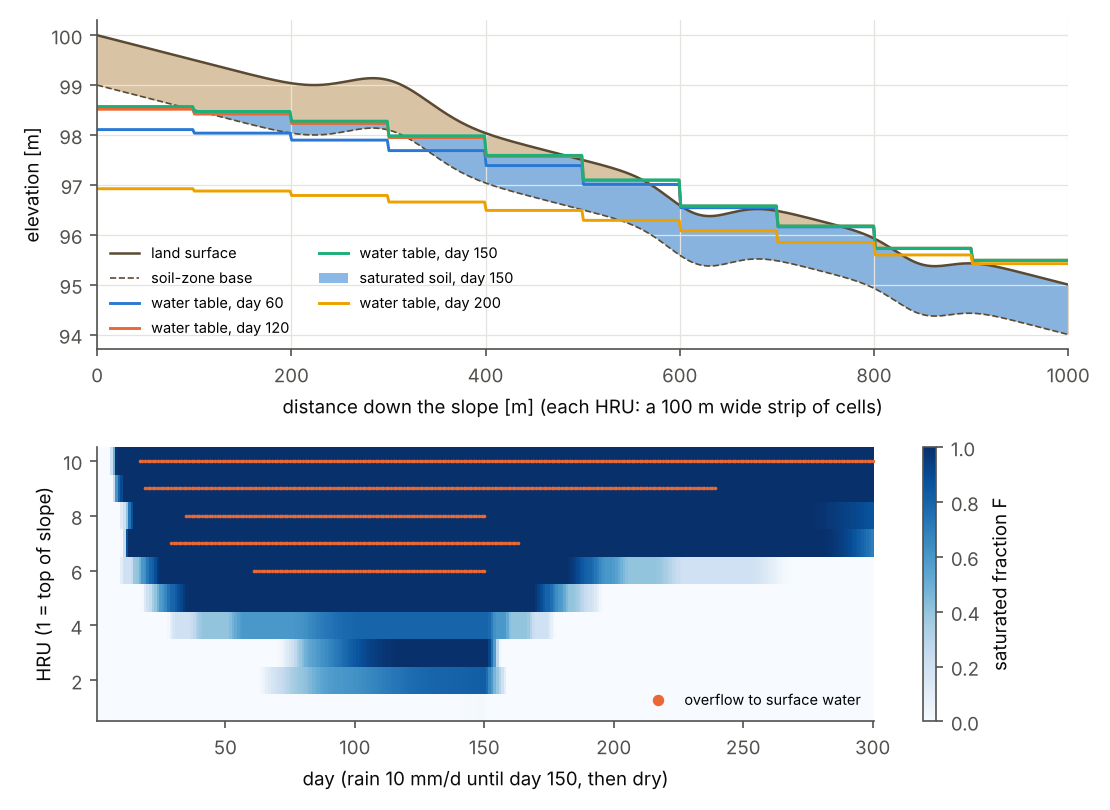
\includegraphics[width=\linewidth]{figures/fig_sz_hillslope.png}
\caption{Coupled hillslope with irregular land (rain 10~mm/d for 150 days, then dry). Top: land surface, soil-zone base and
the water table of each cell on four days; shaded, the saturated soil on day 150. Bottom: saturated fraction $F$ of each
HRU over time (1 = top of the slope), with the days on which the HRU overflows to surface water.}\label{fig:uszhillslope}
\end{figure}
\item \textbf{A deep water table elsewhere}: \cmd{:SoilZoneVadose RICHARDS} (or \cmd{KINEMATIC}, \cmd{LAG}) carries the
recharge through the unsaturated zone between the soil and the water table, with its delay (Section~\ref{sec:uvadose}).
On hummocky ground \cmd{:SoilZoneVadoseClasses} 3 gives the hollows and the hummocks their own columns (Reference,
Section~\ref{R-sec:vzclasses}). Capillary rise from a shallow water table is then on by default. Reference,
Figure~\ref{R-fig:szregimes}, shows every position of the water table and what carries the water in each; the coupling
moves between them without any setting.
\item \textbf{HRUs that are wet at the foot and dry at the top}: \cmd{:SoilZoneClasses} 3--5 runs Raven's processes on
classes of an HRU's columns (needs \cmd{:Method ORDERED\_SERIES}).
\item \textbf{Check}: \cmd{GWSoilExchange.csv} gives, per HRU and step, the soil-zone base, the soil water level, the water
table and the saturated fraction $F$; \cmd{tools/plot\_soilzone.py} plots them, and \cmd{tools\_audit.py} closes every
soil-zone identity. The interface should converge on every step (\cmd{GWBudget.csv}, \emph{interface converged}).
\end{enumerate}
The coupling has been checked on planar and irregular hillslopes against a MODFLOW-only reference (Reference,
Section~\ref{R-sec:vszbasic}) and on 400 randomly drawn rough-terrain cases (1\,620 runs with the four unsaturated-zone
methods and the regression cases) with slopes up to 30\,\%, pits, cliffs, ridges, sloping and pinching layers and DEMs
coarser or finer than the grid (Reference, Section~\ref{R-sec:vrough}). The reference for every command is Reference,
Table~\ref{R-tab:szcmds}. Workshop~3 takes you through these steps.

\subsection{The unsaturated zone: NONE, RICHARDS, KINEMATIC or LAG}\label{sec:uvadose}
When the water table lies well below the soil, rain that drains out of the soil takes days to weeks to reach it, and
arrives spread out. \cmd{:SoilZoneVadose} chooses how that trip through the dry ground is computed. It applies only with
\cmd{:SoilZone PHYSICAL}.
\begin{table}[!htbp]\centering
\caption{The four methods of \cmd{:SoilZoneVadose}.}\label{tab:uvadose}
\begin{tabularx}{\linewidth}{P{0.17\linewidth}P{0.37\linewidth}Y}\toprule\hdr
Method & What it does & Use it when\\\midrule
\cmd{NONE} (default) & recharge reaches the water table in the step & the water table is shallow, or the timing of recharge does not matter\\
\cmd{RICHARDS} & Richards' equation on a column of nodes, from the soil's retention curve; capillary rise also from the column & the reference method: the timing matters and the materials are known\\
\cmd{KINEMATIC} & Richards' equation without capillary forces (as MODFLOW's UZF package and GSFLOW) & a delay that depends on the flux, at a fraction of the cost; it cannot fail to converge\\
\cmd{LAG} & a cascade of linear stores with a travel time per metre $t_m$ & only the delay and spreading matter; $t_m$ is the one parameter to calibrate (0: derived from each material)\\\bottomrule
\end{tabularx}
\end{table}
\begin{whattowrite}
\cmd{:SoilZoneVadose RICHARDS}\quad or\quad \cmd{:SoilZoneVadose KINEMATIC}\quad or\quad \cmd{:SoilZoneVadose LAG 2}\\
\cmd{:SoilZoneVadoseClasses 3}\quad (optional: hollows and hummocks get their own columns)
\end{whattowrite}
The columns use \cmd{POROSITY}, \cmd{CLAPP\_B} and \cmd{AIR\_ENTRY\_PRESSURE} of the aquifer classes (defaults 0.3, 4
and 0.3~m; for an existing model, those of \cmd{:SoilZoneAquiferClass}).

\begin{example}[: a storm over a deep water table]
A 3-day storm of 40~mm/d on soil over a water table 6~m deep, in sand (test P1 of the Reference). Without a column the
recharge reaches MODFLOW with the percolation, centred on day~6.1. With \cmd{RICHARDS} it arrives spread over two weeks,
its peak 45\% lower, centred on day~15.6. With \cmd{LAG 2} the centre is on day~13.9, with \cmd{LAG 4} on day~21.1.
Nothing is lost in any of them.
\end{example}

Figures~\ref{fig:uvzkinematic} and \ref{fig:uvzlag} show how \cmd{KINEMATIC} and \cmd{LAG} delay and spread the
recharge, and Figure~\ref{fig:uvzclasses} how \cmd{:SoilZoneVadoseClasses} groups the low and high parts of a cell.
\begin{figure}[!htbp]\centering
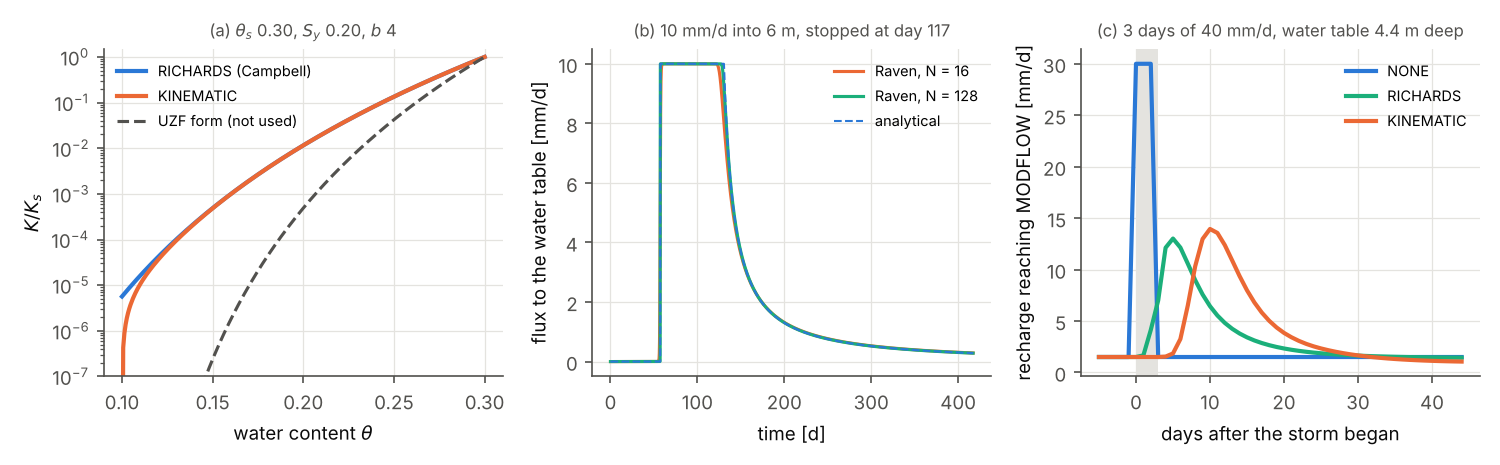
\includegraphics[width=\textwidth]{figures/fig_vz_kinematic.png}
\caption{\cmd{KINEMATIC}. (a) How the ground's conductivity grows as it gets wetter, compared with the curve \cmd{RICHARDS} uses. (b) Rain of 10~mm/d for 117 days over a water table 6~m down: the water reaching the water table, against the exact solution. (c) A 3-day storm over a deep water table: the recharge arrives later and spread out.}\label{fig:uvzkinematic}
\end{figure}
\begin{figure}[!htbp]\centering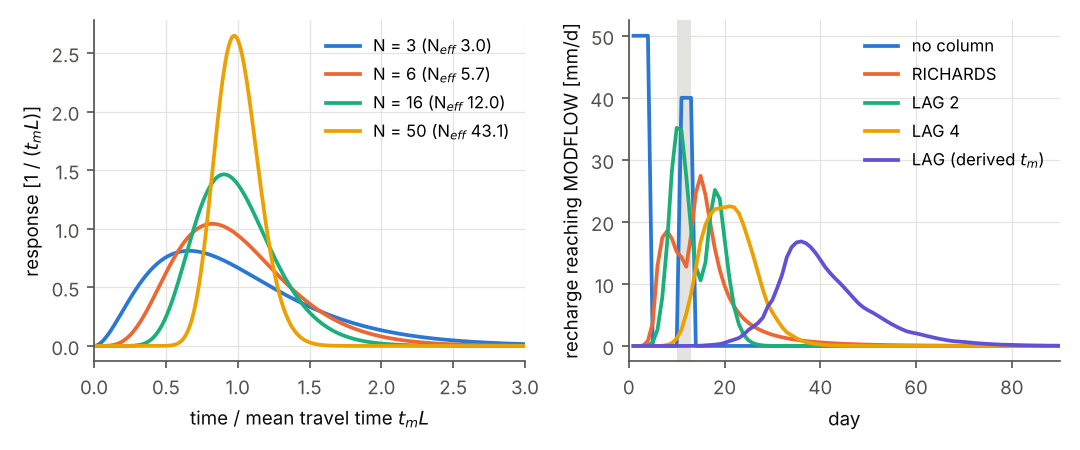
\includegraphics[width=\linewidth]{figures/fig_vz_lag_cascade.png}
\caption{\cmd{LAG}. Left: water entering the top of a column comes out at the bottom spread over time; more nodes give a sharper peak. Right: the recharge from a 3-day storm reaching a water table 6~m down, without a column, with \cmd{RICHARDS} and with \cmd{LAG}.}\label{fig:uvzlag}
\end{figure}
\begin{figure}[!htbp]\centering
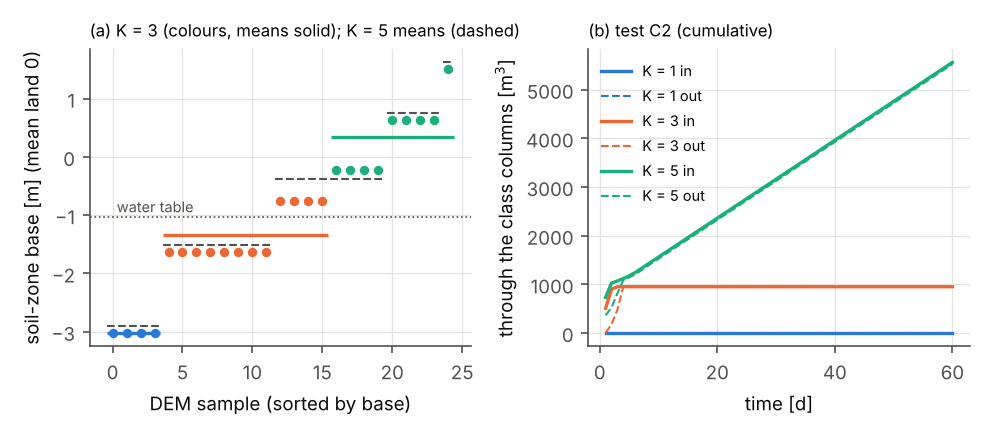
\includegraphics[width=\linewidth]{figures/fig_vz_classes.png}
\caption{Depth classes. (a) The 25 sample points of a hummocky cell, sorted by depth and grouped into 3 classes (colours) or 5; each class gets its own column. (b) The water entering and leaving the class columns in a test, summed over time.}\label{fig:uvzclasses}
\end{figure}
\paragraph{Capillary rise.} When the water table is shallow, dry soil also pulls water up from it, so plants and
evaporation keep drawing on groundwater after the rain stops. \cmd{:SoilZoneCapillaryRise} is \cmd{ON} by default with
\cmd{RICHARDS}, \cmd{KINEMATIC} and \cmd{LAG}, and \cmd{OFF} with \cmd{NONE}. It is computed from the soil's own retention
curve, not from a fitted rate.

\paragraph{Cost.} On the Liard example with \cmd{:SoilZone PHYSICAL} (85 HRUs, one year) the run takes 69~s with the
defaults, and 91~s with unsaturated columns, capillary rise and three classes. MODFLOW's solve remains the larger part.

\section{Common questions}
\paragraph{Can only part of my watershed have groundwater?} Yes. Only HRUs with an \cmd{AQUIFER\_PROFILE} are coupled; all
others run exactly as they do without groundwater.
\paragraph{Can two aquifer systems exchange water?} Yes, when their cells touch: lateral flow between neighbouring profiles
and leakage between layers are computed by MODFLOW like any other flow.
\paragraph{What happens where the water table reaches the surface?} The seepage drains return the water to Raven, where it
follows Raven's processes (for example baseflow to the river).
\paragraph{Can the aquifer take more water than a river carries?} Not from a river Raven builds: the supply limit caps
each river cell's largest possible loss at its share of the reach's flow at the start of the step, and the loss is taken
from the reach's runoff, inflow and outflow, so the outflow leaving the watershed falls by it. Only a reach whose flow stops
within the step can leave part of its loss to be carried to the next step (warned about; the loss carried at the end of
the run is a run total of \cmd{GWModelSummary.txt}). An existing model's stream package keeps its own conductance and has
no supply limit (Reference, Section~\ref{R-sec:extlimits}): a losing reach can take more than the channel holds, and the
part the channel cannot supply is carried to the next step (\emph{river loss carried to next step}; exactly accounted).
Example~B does this for months: the carry reaches about $10^{8}$~m$^3$ and is repaid by the end of the run.
\paragraph{Does frozen ground limit recharge?} Recharge is whatever Raven's processes send to \cmd{GROUNDWATER}, so frozen
ground acts on it through Raven's own process choices (a \cmd{:FrozenGround} process, infiltration and percolation methods
that respond to frozen soil); the coupling adds no frozen-ground control of its own.
\paragraph{Does the coupling change results for my other subbasins?} Only through the rivers: groundwater discharge or
losses in coupled subbasins change the flow passed downstream.
